\begin{figure*}[t]
    \centering
    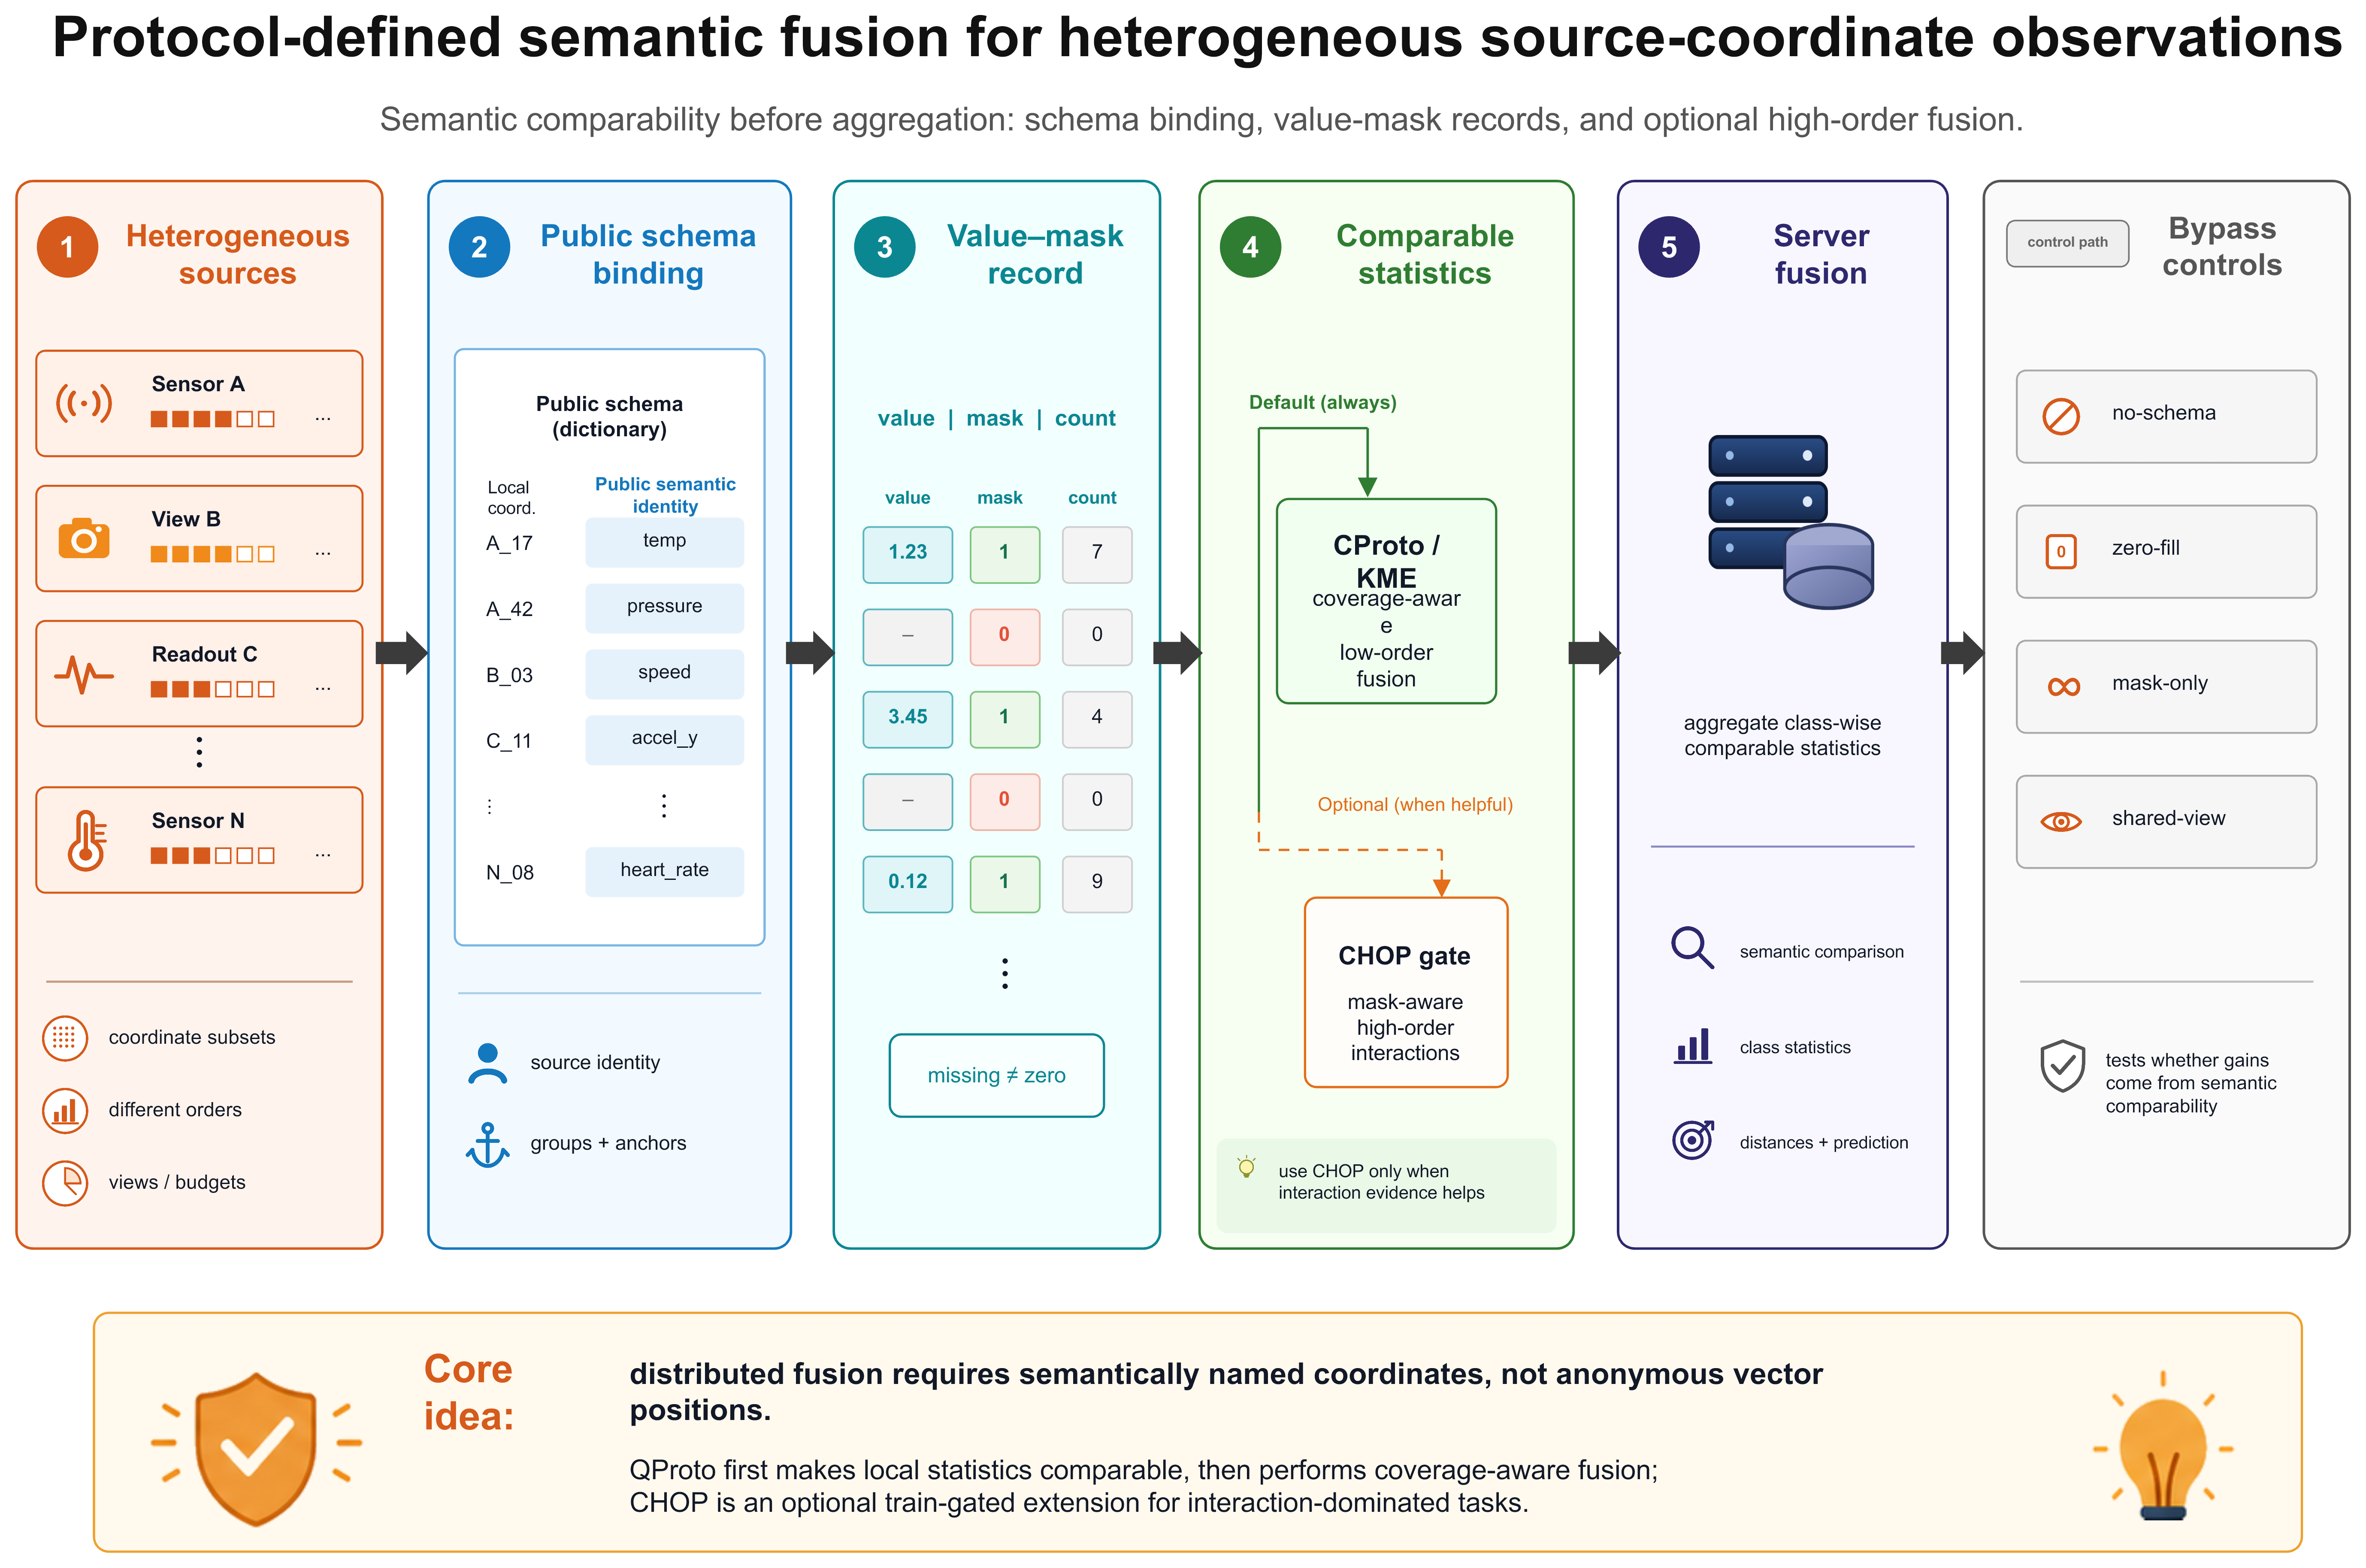
\includegraphics[width=\textwidth]{figures/fig1_semantic_fusion_redrawn_v45_cropped.png}
    \caption{Protocol-defined semantic fusion for heterogeneous source-coordinate observations. Local sources may expose different coordinate subsets, orders, views, noise levels, or measurement budgets. \method\ first binds local coordinates to public semantic identities, then maps observations into value-mask records with coverage counts so that missing measurements are not confused with measured near-zero values. The default path performs low-order coverage-aware CProto/KME fusion, while CHOP is a train-gated high-order extension used only when interaction evidence helps. Bypass controls test whether gains come from semantic comparability rather than anonymous vector averaging.}
    \label{fig:if-framework}
\end{figure*}



